\documentclass[border=10pt]{standalone}
\usepackage{pgfplots}
\pgfplotsset{compat=1.18}

\begin{document}
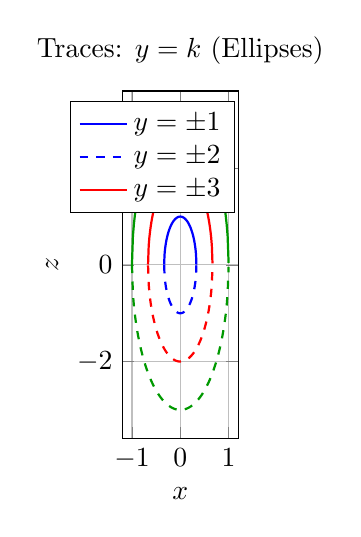
\begin{tikzpicture}
\begin{axis}[
    xlabel={$x$},
    ylabel={$z$},
    title={Traces: $y = k$ (Ellipses)},
    domain=-1:1,
    samples=100,
    grid=major,
    width=8cm,
    height=6cm,
    axis equal image,
    legend pos=north east
]
% Ellipses for y = 1, 2, 3
% 9x^2 + z^2 = k^2 => z = +/- sqrt(k^2 - 9x^2)
\addplot[blue, thick, domain=-1/3:1/3] {sqrt(1 - 9*x^2)};
\addplot[blue, thick, dashed, domain=-1/3:1/3] {-sqrt(1 - 9*x^2)};
\addlegendentry{$y = \pm 1$}

\addplot[red, thick, domain=-2/3:2/3] {sqrt(4 - 9*x^2)};
\addplot[red, thick, dashed, domain=-2/3:2/3] {-sqrt(4 - 9*x^2)};
\addlegendentry{$y = \pm 2$}

\addplot[green!60!black, thick, domain=-1:1] {sqrt(9 - 9*x^2)};
\addplot[green!60!black, thick, dashed, domain=-1:1] {-sqrt(9 - 9*x^2)};
\addlegendentry{$y = \pm 3$}
\end{axis}
\end{tikzpicture}
\end{document}